\documentclass{article}
\usepackage{tikz, pgfplots, amsmath, amsthm, amsfonts}
\usepackage{subcaption}
\begin{document}

\section{Chapter 1: Graphs and Subgraphs}
\subsection{Graphs and Simple Graphs}
%\subsubsection{}

\indent{} Graphs are the collections of three sets: Vertices, Edges, and the incidence function. The incidence function is the way of 'mapping' an edge to a vertex.
Denote Vertices as $V(G)$, Edges as $E(G)$, and the incidence function as $\Psi(G)$.
\newline
Take $G$ as a graph. This can be represented as the ordered triple like:
\[G = (V(G), E(G), \Psi(G))\]

If we look at the incidence function, we can look at two vertices, $u,v$ and an edge $e$. $e$ is said to join the vertices if:
\[\Psi_G(e) = uv \] 
\indent{} $u,v$ are said to be the ends of the edge $e$. This is an example of the graph with the function of:
\begin{align*}
    \Psi_H(a) = uv, && \Psi_H(b) = uu, && \Psi_H(c) = vw, && \Psi_H(d) = wx\\
    \Psi_H(e) = vx, && \Psi_H(f) = wx, && \Psi_H(g) = ux, && \Psi_H(h) = xy
\end{align*}

This is the incidence function. The edge set and vertex set look like:
\begin{align*}
    &V(H) = \left\{u,v,w,x,y\right\}\\
    &E(H) = \left\{a,b,c,d,e,f,g,h\right\}
\end{align*}

\begin{figure}[ht]
    \centering
    
    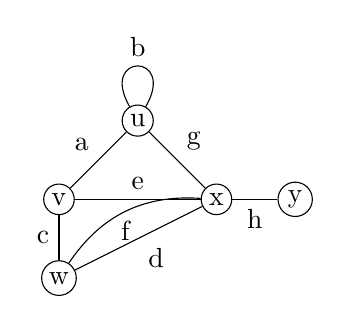
\begin{tikzpicture}
        % Nodes
        \node[circle, draw, fill=white, inner sep=1.5pt] (v) at (0,0) {v};
        \node[circle, draw, fill=white, inner sep=1.5pt]  (u) at (1,1) {u};
        \node[circle, draw, fill=white, inner sep=1.5pt]  (w) at (0,-1) {w};
        \node[circle, draw, fill=white, inner sep=1.5pt]  (x) at (2,0) {x};
        \node[circle, draw, fill=white, inner sep=1.5pt] (y) at (3,0) {y};
        
        % Edges
        \draw (v) -- (u) node[midway, above left] {a};
        \draw (v) -- (w) node[midway, left] {c};
        \draw (v) -- (x) node[midway, above] {e};
        \draw (u) -- (x) node[midway, above right] {g};
        \draw (w) -- (x) node[midway, below right] {d};
        \draw (x) -- (y) node[midway, below] {h};
        
        % Loops
        \draw[loop above] (u) to[out=120, in=60, looseness=10] node[above] {b} (u);
        \draw[bend right] (x) to[out=-30, in=-150] node[midway, below] {f} (w);
    \end{tikzpicture}
    \caption{}
\end{figure}

There are two types of graphs \emph{planar} and \emph{nonplanar}. Planar means that the graph can be represented such that no edges intersect at all (except the ends of course). A nonplanar follows to mean the opposite.
A non-planar graph is shown below:

\begin{figure}[ht]
    \centering
    
    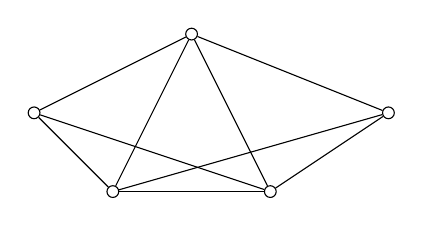
\begin{tikzpicture}
        %nodes
        \node[circle, draw, fill=white, inner sep=1.5pt] (a) at (1, 0) {};
        \node[circle, draw, fill=white, inner sep=1.5pt] (b) at (2.5, 1) {};
        \node[circle, draw, fill=white, inner sep=1.5pt] (c) at (0, 2) {};
        \node[circle, draw, fill=white, inner sep=1.5pt] (d) at (-2, 1) {};
        \node[circle, draw, fill=white, inner sep=1.5pt] (e) at (-1, 0) {};

        %edges
        \draw (a) -- (b) node[midway, above right] {};
        \draw (b) -- (c) node[midway, left] {};
        \draw (c) -- (d) node[midway, left] {};
        \draw (d) -- (e) node[midway, below right] {};
        \draw (e) -- (a) node[midway, right] {};

        %inner edges
        \draw (a) -- (c) node[midway, above] {};
        \draw (e) -- (c) node[midway, above] {};
        \draw (a) -- (d) node[midway, above left] {};
        \draw (e) -- (b) node[midway, above right] {};
    \end{tikzpicture}
    \caption{}
\end{figure}

\indent{} As one can see, the intersecting lines in the middle there are way makes this graph nonplanar. If there was a way to draw the graph without the intersecting edges, then it would be planar.
\newline
\indent{} The ends of an edge are said to be \emph{incident} with the edge. Two vertices that share an edge (ie incident) are said to be \emph{adjacent}. An edge that connects a vertex to itself is a \emph{loop}. An edge with distinct ends is a \emph{link}.
\newline
\indent{} A graph is said to be \emph{finite} if both the vertex and edge set are finite. For the sake of the book, we only work with finite and also any graph with just one vertex is said to be \emph{trivial} while any more is nontrivial.
\newline
\indent{} A graph is said to be \emph{simple} if it has no loops and no two links join the same pair of vertices. Figure 1 is not simple because of the joining of edge $d$ and edge $f$ to the same vertex from the same origin vertex.
Figure 2 however, is also not simple because multiple edges between vertices exist. A simple graph can be like:
\begin{figure}[ht]
    \centering
    \begin{tikzpicture}
        %nodes
        \node[circle, draw, fill=white, inner sep=1.5pt] (a) at (0, 0) {};
        \node[circle, draw, fill=white, inner sep=1.5pt] (b) at (1, -1) {};
        \node[circle, draw, fill=white, inner sep=1.5pt] (c) at (-1, -2) {};
        \node[circle, draw, fill=white, inner sep=1.5pt] (d) at (1, 2) {};

        %edges
        \draw (a) -- (b) node[midway, above] {};
        \draw (b) -- (c) node[midway, above] {};
        \draw (c) to [out=135, in=90, looseness=1] (d) {};
        \draw (c) -- (a) {};
        \draw (d) -- (a) {};
    \end{tikzpicture}
    \caption{Simple Graph}
\end{figure}
\newline

\subsection{Graph Isomorphisms}
\indent{} Two graphs are \emph{identical} assuming that the edge set, vertex set, and incidence function are all equal to each other ($G=H$). Now, if we have two graphs that are of the same diagram, but are not identical. Look at the below figure we call these \emph{isomorphic}.

\begin{figure*}[ht]
    \begin{subfigure}{0.45\textwidth}
        \centering
        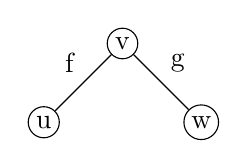
\begin{tikzpicture}
            %nodes
            \node[circle, draw, fill=white, inner sep=1.5pt] (a) at (0, 0) {v};
            \node[circle, draw, fill=white, inner sep=1.5pt] (b) at (-1, -1) {u};
            \node[circle, draw, fill=white, inner sep=1.5pt] (c) at (1, -1) {w};

            %edges
            \draw (a) -- (b) node[midway, above left] {f};
            \draw (a) -- (c) node[midway, above right] {g};
        \end{tikzpicture}
        \caption{G graph}
    \end{subfigure}%
    %
    \begin{subfigure}{0.45\textwidth}
        \centering
        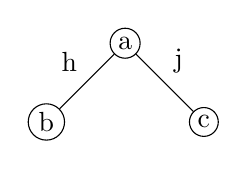
\begin{tikzpicture}
            %nodes
            \node[circle, draw, fill=white, inner sep=1.5pt] (a) at (0, 0) {a};
            \node[circle, draw, fill=white, inner sep=1.5pt] (b) at (-1, -1) {b};
            \node[circle, draw, fill=white, inner sep=1.5pt] (c) at (1, -1) {c};

            %edges
            \draw (a) -- (b) node[midway,  above left] {h};
            \draw (a) -- (c) node[midway,  above right] {j};
        \end{tikzpicture}
        \caption{H graph}
    \end{subfigure}%
    %\
\end{figure*}

\indent{} These are considered isomorphic ($G \cong H$) because the vertex sets are (obviously) not equal, but they are otherwise the same diagram. We call two graphs isomorphic if
there exist a bijection $\theta: V(G) \mapsto V(H)$, and $\phi: E(G) \mapsto E(H)$.
This means:
\[\Psi_G(e) = uv \iff \Psi_H(\phi(e)) = \theta(u)\theta(v)\]
For the two graphs above, we can look at the maps as:
\begin{align*}
    \theta(u) = b, && \theta(v) = a, && \theta(w) = c
\end{align*}
the mappings for the edges then are:
\begin{align*}
    \phi(f) = h, && \phi(g) =j
\end{align*}
\indent{} This can be represented as a pair of mappings like: $(\theta, \phi)$. This is one of those things that is useful, but for the sake of the book, most graphs are probably going to be not labeled.
In this sense, we can think of the unlabelled graphs as representatives of an equivalence class of isomorphic graphs.
\newline
\indent{} A simple graph where each pair of distinct vertices is joined by an edge is a \emph{complete graph} (ie no vertex has no edge). Yes, an isomorphism can exist between two non-complete graphs. An \emph{empty graph} is one with no edges. A \emph{bipartite graph} is one where
the vertex set can be partitioned into two subsets $X$, $Y$. The partition allows it so that each edge has one end in $X$ and another in $Y$. This partition, ($X, Y$) is called a \emph{bipartition} of the graph. Extending this further, a \emph{complete bipartite graph} is a simple bipartite graph with a bipartition ($X, Y$) where each vertex of $X$ is joined to each vertex of $Y$.
if $\left|X\right| = m$ and $\left|Y\right| = n$ we denote this as: $K_{m,n}$.
\newline
\indent{} Examples of bipartite and complete bipartite are below:

\begin{figure}[ht]
    \begin{subfigure}{0.45\textwidth}
        \centering
        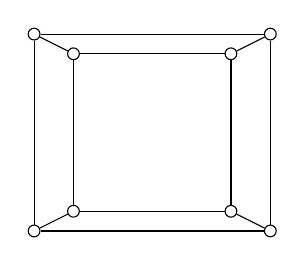
\begin{tikzpicture}
            %nodes
            \node[circle, draw, fill=white, inner sep =1.5pt] (a) at (1, 1) {};
            \node[circle, draw, fill=white, inner sep =1.5pt] (b) at (1, -1) {};
            \node[circle, draw, fill=white, inner sep =1.5pt] (c) at (-1, 1) {};
            \node[circle, draw, fill=white, inner sep =1.5pt] (d) at (-1, -1) {};
            \node[circle, draw, fill=white, inner sep =1.5pt] (e) at (1.5, 1.25) {};
            \node[circle, draw, fill=white, inner sep =1.5pt] (f) at (1.5, -1.25) {};
            \node[circle, draw, fill=white, inner sep =1.5pt] (g) at (-1.5, 1.25) {};
            \node[circle, draw, fill=white, inner sep =1.5pt] (h) at (-1.5, -1.25) {};
            
            %edges
            \draw (a) -- (b) {};
            \draw (a) -- (c) {};
            \draw (b) -- (d) {};
            \draw (d) -- (c) {};
            \draw (a) -- (e) {};
            \draw (b) -- (f) {};
            \draw (c) -- (g) {};
            \draw (d) -- (h) {};
            \draw (f) -- (h) {};
            \draw (e) -- (f) {};
            \draw (e) -- (g) {};
            \draw (h) -- (g) {}; 
        \end{tikzpicture}
        \caption{Bipartite}
    \end{subfigure}%
    \begin{subfigure}{0.45\textwidth}
        \centering
        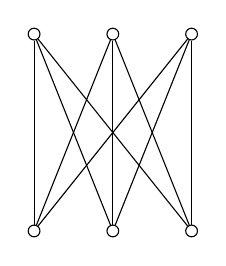
\begin{tikzpicture}
            %nodes
            \node[circle, draw, fill=white, inner sep=1.5pt] (a) at (-1, 1.5) {};
            \node[circle, draw, fill=white, inner sep=1.5pt] (b) at (0, 1.5) {};
            \node[circle, draw, fill=white, inner sep=1.5pt] (c) at (1, 1.5) {};
            \node[circle, draw, fill=white, inner sep=1.5pt] (d) at (-1, -1) {};
            \node[circle, draw, fill=white, inner sep=1.5pt] (e) at (0, -1) {};
            \node[circle, draw, fill=white, inner sep=1.5pt] (f) at (1, -1) {};

            %edges
            \draw (a) -- (f) {};
            \draw (a) -- (d) {};
            \draw (a) -- (e) {};
            \draw (b) -- (f) {};
            \draw (b) -- (e) {};
            \draw (b) -- (d) {};
            \draw (c) -- (f) {};
            \draw (c) -- (e) {};
            \draw (c) -- (d) {};
        \end{tikzpicture}
        \caption{Complete Bipartite}
    \end{subfigure}
\end{figure}
Note to the reader: See where you can create a line between the Vertices. You'll see if you can split it into halves you might see your $X$ and $Y$ sets just from inspection.

\subsection{The Incidence and Adjacency Matrices}
\end{document}